\subsection{Web Browser Support}

\autoref{tab:browser-support} shows the web browser support status of the \wa{}, both for desktop and mobile web browser, and if they support the \gls{api}. If so, the table shows the version which initially added support for the \wa{} alongside with the release date. The following subsections will explain the web browser support more detailed.

The global web browser support as of August 2019 adds up around 70\%, given the fact that web browser usage statistics vary between services.\footcites[The obtained data is available in the Appendix \autoref{sec:stats}, see][]{statcounter-global}

\newpage

\begin{table}[ht]
	\begin{tabularx}{\textwidth}{l|p{5.3cm}|p{2cm}|p{1.7cm}|p{3.08cm}}
		& Web browser & Supported & Version & Release Date \\
		\hline
		\parbox[t]{2mm}{\multirow{6}{*}{\rotatebox[origin=c]{90}{Desktop}}} & Chrome & \OK & 67 & May 2018 \\
		& Firefox & \OK & 60 & May 2018 \\
		& Opera & \OK & 54 & June 2018 \\
		& Internet Explorer & \NOOK & - & - \\
		& Edge & \OK & 18 & November 2018 \\
		& Safari & \OK & 13 & September 2019 \\
		\hline
		\parbox[t]{2mm}{\multirow{6}{*}{\rotatebox[origin=c]{90}{Mobile}}} & Opera Mobile & \NOOK & - & - \\
		& IE Mobile & \NOOK & - & - \\
		& Safari (iOS) & \NOOK & - & - \\
		& Google Chrome (iOS) & \NOOK & - & - \\
		& Firefox (iOS) & \NOOK & - & - \\
		& Brave (iOS) & \OK & 1.11.3 & August 2019 \\
		\hline
		\parbox[t]{2mm}{\multirow{14}{*}{\rotatebox[origin=c]{90}{Android}}} & LineageOS Stock Browser & \NOOK & - & - \\
		& Chrome for Android & \OK & 70 & October 2018 \\
		& Firefox for Android (Fennec) & \OK & 68 & July 2019 \\
		& Firefox Preview (Fenix) & \NOOK & - \\
		& Opera & \NOOK & - & - \\
		& Opera mini & \NOOK & - & - \\
		& Edge & \NOOK & - & - \\
		& Samsung Internet & \NOOK & - & - \\
		& UC Browser & \NOOK & - & - \\
		& Mint Browser & \NOOK & - & - \\
		& 360 Secure Browser & \NOOK & - & - \\
		& QQ Browser & \NOOK & - & - \\
		& Yandex Browser & \NOOK & - & - \\
		& Brave Browser & \NOOK & - & -
	\end{tabularx}
	\caption[Web browser support of the \wa]{Web browser support of the \wa\footnotemark}
	\label{tab:browser-support}
\end{table}
\footcitetexts[Sources:][]{chrome-webauthn}{firefox-webauthn}{safari-webauthn}{chrome-android-webauthn}[a detailed analysis of Android web browsers is available on the \gls{usb} flash drive in the appendix.]{firefox-android-webauthn}

\subsubsection{Desktop Support}

The \wa{} is supported from Chrome 67 onwards, which was released in May 2018. Firefox added support for the \wa{} in May 2018 with its version 60 as well.\\
Microsoft added support for the \wa{} in Edge 13 which was released in November 2015. However, the implementation is based on an earlier draft version of the \wa. Support for the \gls{fido} 2.0 specification was added in Edge 14 (released in December 2016). The feature is hidden behind a configuration option though and was enabled for all users with the release of Edge 17 in November 2018.\footcite[See][112]{Jacobs:2019}

Web browsers such as Opera, Vivaldi, Brave, and upcoming Edge versions that are all based on Chromium, the web browser and source code behind Google's Chrome web browser, have support for the \wa, too.\footcites[See][Chapter 7.1]{kissell2019take}

As the development for the Internet Explorer halted, and it is only receiving security updates, no support is available for new web \glspl{api} including the \wa. Even though it is still used by over 4\% of all desktop web browser users and remains supported for the operating system Windows 7, 8.1 and 10. This is an important fact to take into account when evaluating the usability of the \wa{} since especially enterprise users often cannot upgrade or switch their web browser.\footcites[See][]{ie-support}[See][]{statcounter-desktop}

Safari added support for the \wa{} feature in December 2018 but only for the preview variant of the web browser, called the Safari Technology Preview. On September 20 Safari 13 was released for the \gls{os} versions macOS High Sierra and Mojave. The support is limited to \gls{usb}-HID enabled authenticators though.\footcites[See][]{safari-webauthn}[See][]{safari-13-release}

Besides that, Windows 10 also added support for \gls{mfa} by incorporating the technology described in the \gls{fido}2 standard. This allows biometric authentication with, e.g., fingerprints when a reader is available or to use the facial recognition technology or iris scans. The feature is called \frqq Windows Hello\flqq{}. Credentials are only stored locally and are protected by asymmetric encryption. Besides biometric authentication Windows Hello also supports \glspl{pin}. The \gls{tpm} stores this \gls{pin}. Windows Hello can be used in desktop web browsers, i.e., delegating the \wa{} functionality to the \gls{os}.\footcites[See][]{201612}[See][6]{fido-whitepaper-amd}

\subsubsection{Mobile Support}

The support for the \wa{} in mobile web browsers is inferior to the desktop support. While Chrome for Android supports the \wa{} since October 2018 and Firefox since July 2019, stock iOS completely lacks support for the \wa. Even though in the iOS 13 settings the feature can be enabled in the \frqq Experimental Features\flqq{} section, the \gls{api} remains unsupported or at least there is no way to add an authenticator in the web browser yet.\footcites[See][]{chrome-android-webauthn}[See]{firefox-android-webauthn}

The only ray of hope is that the Brave web browser for iOS added support for the security key \frqq YubiKey 5Ci\flqq{} which enables the \wa{} for iOS by using an Apple certified Lightning accessory. \autoref{fig:brave_success} shows a successful authentication with the YubiKey 5Ci and the Brave web browser for iOS. iPad devices with a \gls{usb}-C connector currently do not work yet. Further, the YubiKey 5Ci is not recognized in the Safari web browser, too.\footcites[See][]{brave-ios}[See][]{brave-now-available}[See][]{fido-ct-6}

\begin{figure}[hbt]
	\centering
	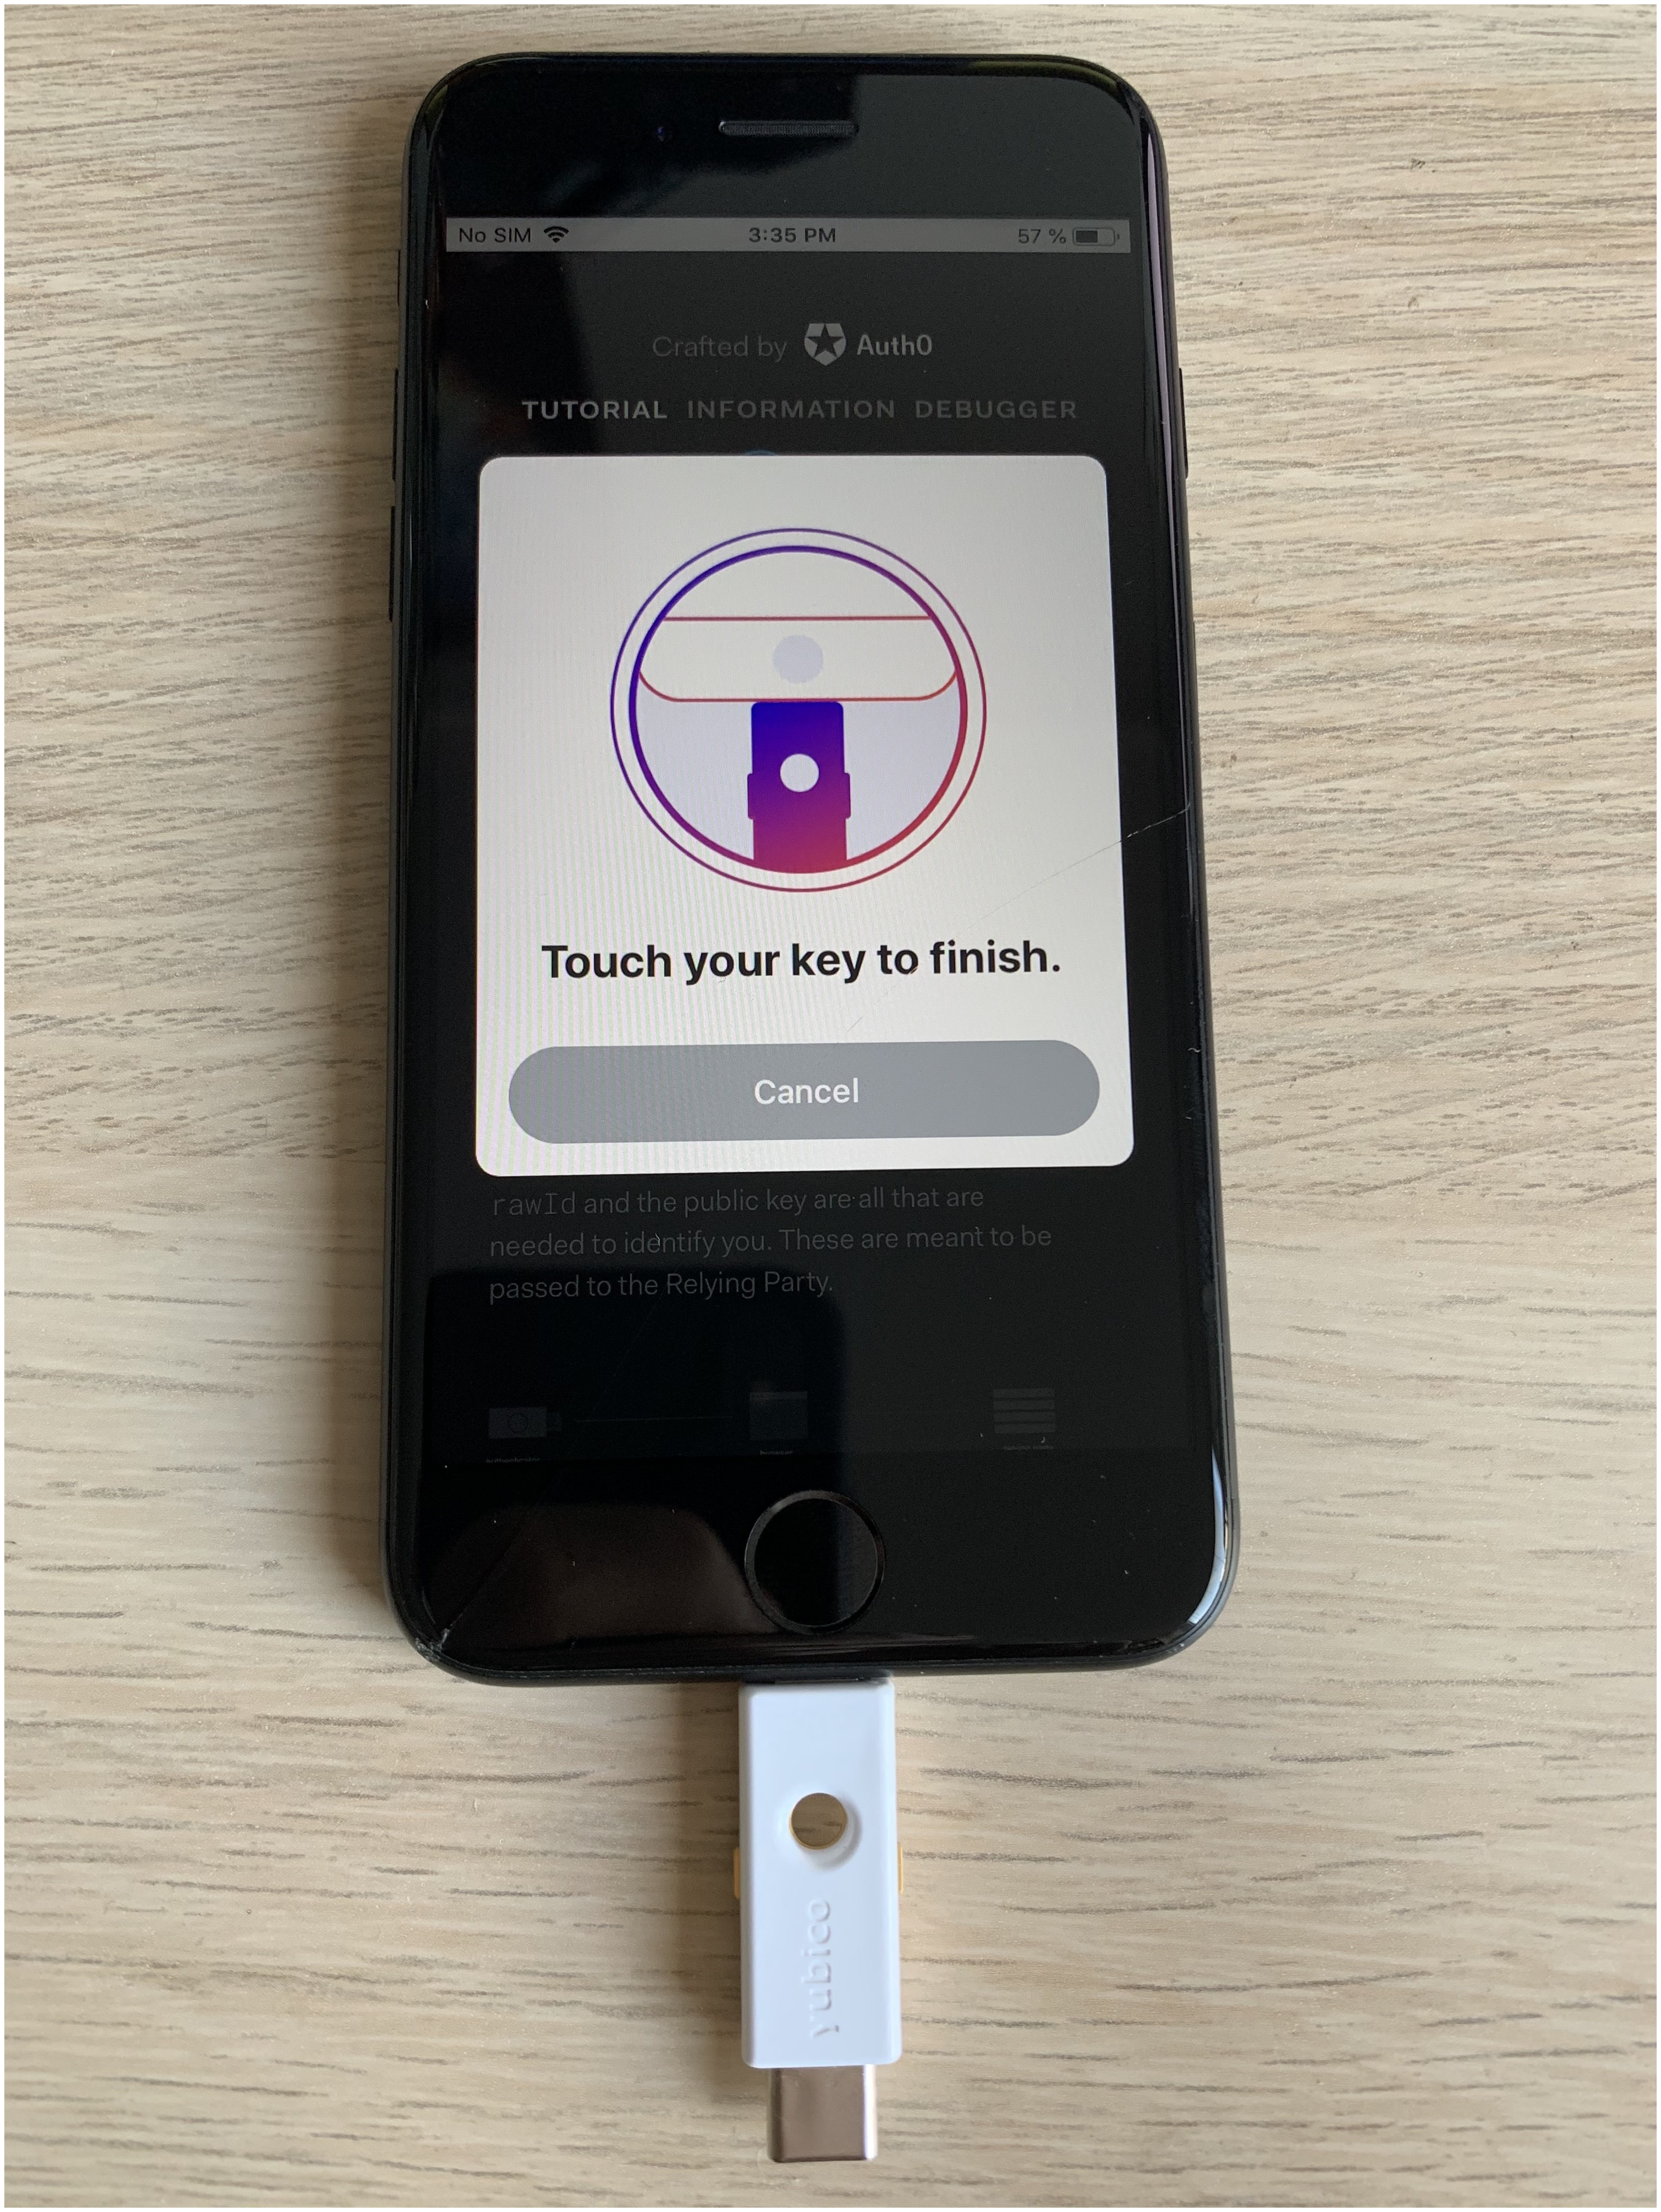
\includegraphics[width=0.6\textwidth]{pics/brave_success_5ci.eps}
	\caption[Successful use of the \wa{} with the Brave web browser on an iPhone 7 with the YubiKey 5Ci]{Successful use of the \wa{} with the Brave web browser on an iPhone 7 with the YubiKey 5Ci\footnotemark}
	\label{fig:brave_success}
\end{figure}
\footnotetext{Source: author's own photograph}

However, \autoref{fig:brave_try} shows the try to use an existing Security Key by Yubico with a lightning dongle in the Brave web browser. While the token has power, Brave does not recognize it, neither is it usable. Safari does not show an overlay for the key usage either.

\newpage

\begin{figure}[hbt]
	\centering
	
\includegraphics[width=0.6\textwidth]{pics/brave_try_dongle.eps}
	\caption[Failed try to use the \wa{} with the Brave web browser on an iPhone 6]{Failed try to use the \wa{} with the Brave web browser on an iPhone 6\footnotemark}
	\label{fig:brave_try}
\end{figure}
\footnotetext{Source: author's own photograph}

It has to be noted though, that other Android web browser vendors need to implement the functionality themselves. Other geographic regions use a variety of different web browsers, e.g., the UC Browser, 360 Security Browser, Mint Browser from Xiaomi, or the QQ Browser from Tencent. Neither they, nor web browsers such as Samsung Internet, Opera (mini) for Android, Edge, or the Android Stock web browser are currently supporting the \wa. The current Firefox for Android (codename \frqq Fennec\flqq) web browser is based on Chromium, too, in contrast to the desktop web browser which is powered by Mozilla's own web browser engine Gecko. A new Firefox for Android web browser, currently called Firefox Preview (codename \frqq Fenix\flqq), which uses a mobile compatible version of Gecko, lacks support for the \wa, too. However, Android offers support for FIDO2 as an \gls{api} and the \gls{os} itself is \gls{fido} certified.\footcites[See][24]{fido-ct-3}

Other mobile \glspl{os}, for example, Windows Phone 8, BlackBerry \gls{os}, BlackBerry 10 or KaiOS do not support the \wa. Further live demonstration captures are available on the attached \gls{usb} flash drive in the appendix.

\subsection{Usability}

One of the main goals of the \wa{} is the \frqq it just works\flqq{} feeling, by providing a secure but abstract solution for the end user. The chosen web browser and \gls{os} are responsible for the design of the login and registration windows, often being native overlays, while in contrast the website designs the traditional login masks and forms. In order to maintain a high usability the user should be able to use a variety of tokens, e.g., built in key stores protected by biometrics or an external token that uses \gls{ble}, \gls{nfc}, or a \gls{usb}-A or \gls{usb}-C interface. Unfortunately, the \frqq it just works\flqq{} can not be fullfilled on macOS or iOS yet.

While the desktop variant of Safari at least contains support for the \wa, the \gls{ctap} is only implemented for \gls{usb}-HID based tokens. Unfortunately no indication, for instance an overlay or popup, that indicate the user needs to interact with their authenticator is shown in Safari. Additionally, Firefox only supports \gls{usb}-HID based authenticators on other operating systems than Windows 10.\footcites[See][]{rust-authenticator}

Besides that, external token that contain a vulnerability in their firmware often need to be replaced, making this both a heavy usability loss, as well as increasing security risk when not replacing the affected token. Both Google's Titan Key and YubiKey's were affected in the past and needed to be replaced.\footcites[See][]{yubikey-heise}[See][]{titan-key}

Further, external tokens are exposed to environment and suffer from the same problems such as the regular tokens do.\footnote{See \autoref{sec:tokens}}

An additional usage implication is the recommendation to have at least two registered tokens for each \gls{rp}. In case one token is lost, stolen, damaged or in any other inaccessible the user still possesses a backup token to gain access to their accounts. Moreover, the \wa{} does not specify a way to backup registered credentials. Unfortunately, the different \gls{usb} interfaces and wireless transportations are not supported on all devices and \gls{os} which further decreases the usability and interoperability.\footcites[See][Chapter 13.6]{w3c}[See][15]{das2018johnny}

Also, the fact that different certification levels of security tokens by the \gls{fido} alliance exist does not make it easier for the end user to pick the right security token. Technically unexperienced users may not know the difference between a \gls{u2f} and \gls{fido}2 certified product, even though only the latter is capable of a completely passwordless process. In addition, end users may not be technically experienced enough to understand the differences in the certification levels of the \gls{fido} alliance.\footcites[See][]{fido-certification}

Finally, different studies showed that users struggle to enable \gls{mfa} with roaming tokens due to lack of feedback and guidance from both the \gls{rp} and the web browsers. Built-in platform authenticator might be able to change this challenge.\footcites[See][]{8418643}[See][884]{usabaility-u2f}[See][15]{das2018johnny}